\input ../SlidePreamble
\input ../preamble


\begin{document}

{\Huge

  \centerline{\bf TTIC 31230, Fundamentals of Deep Learning}
  \bigskip
  \centerline{David McAllester, Winter 2018}
  \vfill
  \centerline{The Evidence Lower Bound (the ELBO)}
  \vfill
  \centerline{Variational Autoencoders}
  \vfill
  \vfill

\slide{{\color{red} Big Picture}: Latent Variables}

We are often interested in models of the form

\vfill
$$P_\Phi(y) = \sum_z\;P_\Phi(z)P_\Phi(y|z).$$

\vfill
Note that CTC has this form.

\vfill
Probabilistic grammar models also have this form where $y$ is a sentence and $z$ is a parse tree.

\vfill
Rate-Distortion Autoencoders also have this form where $z$ is the compression of $y$.

\vfill
In these cases the sum over $z$ can be computed exactly.

\slide{{\color{red} Big Picture}: Friendly Distributions}

A distribution $P(u)$ will be called {\bf friendly} if we can both draw samples from it and compute $P(u)$ for any value $u$.

\vfill
$$P_\Phi(y) = \sum_z\;P_\Phi(z)P_\Phi(y|z).$$

\vfill
It is often the case that $P_\Phi(z)$ is friendly, and $P_\Phi(y|z)$ is friendly, but $P_\Phi(y)$ is not friendly (the sum over $z$ is intractible).

\vfill
For example $z$ might be an assignment of truth values to Boolean variables and $y$ might be the value of a fixed Boolean formula $\Phi$.  In this case
determining if $P_\Phi(y) > 0$ is the SAT problem which is NP hard.

\slide{Superpixel Colorization}

\centerline{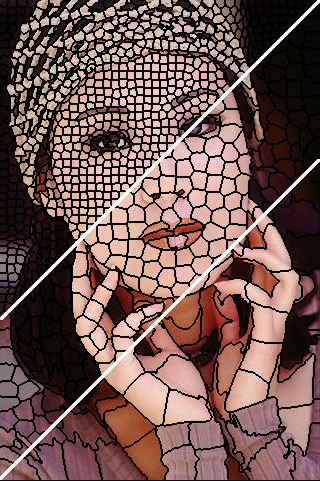
\includegraphics[height = 2in]{../images/SLIC} \hspace{.5in} 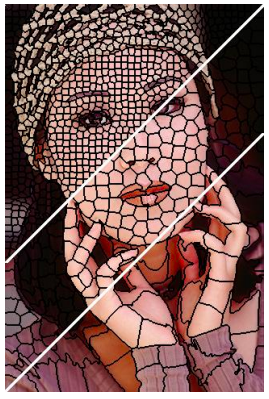
\includegraphics[height = 2in]{../images/SLICcolor}}
\centerline{\huge SLIC superpixels, Achanta et al.}

$x$ is black and white, $y$ color, $z$ a segmentation.

\vfill
$$P_\Phi(y|x) = \sum_z\;P_\Phi(z|x)P_\Phi(y|z,x).$$

\slide{Superpixel Colorization}

$P_\Phi(z|x)$ is defined by a deep network computing a friendly graphical model on segmentations -- perhaps a independent distribution over segment
indeces for each superpixel.

\vfill
$P_\Phi(y|z,x)$ is a deep network taking a particular segmentation (a segment index at each pixel) and computing
a distribution over colors for each segment.

\vfill
Although $P(z|x)$ is friendly, and $P_\Phi(y|z,x)$ is friendly, $P(y|x)$ not friendly (similar to the SAT example).

\slide{{\color{red} Big Picuture}: ELBO Replaces Search with Generation}

\vfill

\begin{eqnarray*}
P_\Phi(y) & = & E_{\color{red} z \sim P_\Phi(z)}P_\Phi(y|z) \;\;\;\mbox{\color{red} sampling $z$ is ineffective}\\
\\
\ln P_\Phi(y) & = & E_{\color{red} z \sim P_\Psi(z|y)} \ln P_\Phi(y) \;\;\;\mbox{\color{red} introduce $z$ generator using $y$}\\
\\
 & = & E_{z \sim P_\Psi(z|y)} \left(\ln P_\Phi(y)P_\Phi(z|y) + \ln \frac{P_\Psi(z|y)}{P_\Phi(z|x)} + \ln\frac{1}{P_\Psi(z|y)}\right) \\
 \\
 \\
 & = & E_{z \sim P_\Psi(z|y)} P_\Phi(z,y) + H(P_\Psi(z|y)) + KL(P_\Psi(z|y),P_\Phi(z|y)) \\
 \\
 & \geq & E_{\color{red} z \sim P_\Psi(z|y)}P_\Phi(z)P_\Phi(y|z) + - \ln P_\Psi(z|y)
\end{eqnarray*}

\slide{Superpixel Colorization}

\centerline{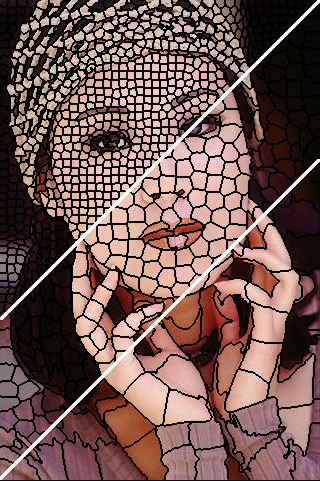
\includegraphics[height = 2in]{../images/SLIC} \hspace{.5in} 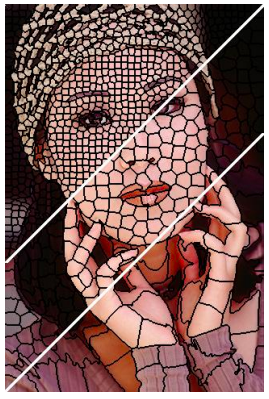
\includegraphics[height = 2in]{../images/SLICcolor}}
\centerline{\huge SLIC superpixels, Achanta et al.}

$x$ is black and white, $y$ color, $z$ a segmentation.

\vfill
$P_\Phi(z|x)$ is friendly and $P_\Phi(y|z,x)$ is friendly but $P(y|x)$ is not friendly.

\vfill
$P_\Psi(z|y,x)$ computes a friendly graphical model for $z$ given $y$.

\slide{Measuring ELBO Loss}

\vfill
$${\cal L}_{\mathrm{ELBO}}(y,\Phi,\Psi)  = E_{z\sim P_\Psi(y)} \; \ln P_\Psi(y) - \ln P_\Phi(z)P_\Phi(y|z)$$

\vfill
If $P_\Phi(z)$, $P_\Phi(y|z)$, and $P_\Psi(z|y)$ are friendly (even whwn when $P_\Phi(y)$ is not friendly) we can
measure ELBO loss through sampling.

\vfill
If we can measure it, we can do gradient descent on it (but perhaps with difficulty).

\slide{A General ELBO Architecture}
\centerline{$P_\Phi(y|x)$ \hspace{10em} $P_\Psi(z|y,x)$}

\parbox{3.5in}{
\begin{eqnarray*}
& & \mbox{intput}\; x \\
\vdots \\
z & = & \expsoftmax_z \ldots \\
\\
& & \mbox{input}\; z \\
\vdots \\
y & = & \expsoftmax_y\;\ldots
\end{eqnarray*}
}
\hfill
\parbox{3.5in}{
\begin{eqnarray*}
& & \mbox{intput}\; x,y \\
\vdots \\
z & = & \expsoftmax_z \ldots \\
\end{eqnarray*}
}

The exponential softmaxes are friendly (they produce a friendly graphical model).

\slide{EM is Alternating Maximization of the ELBO}
Forward-backward EM for HMMs and inside-outside EM for PCFGs (or any EM) can be written as

\vfill
\begin{eqnarray*}
\mathrm{\color{red} ELBO}& = & E_{z \sim P_\Psi(z|y)}\; \ln P_\Phi(z,y) + H(P_\Psi(z|y))\;\;\;(1) \\
 \\      
  & = & \ln\;P_{\Phi}(y) - KL(P_\Psi(z|y),P_{\Phi}(z|y))\;\;\;\;\;\;(2)
\end{eqnarray*}

\vfill
\begin{eqnarray*}
\mbox{by (2)}\;\;\;\Psi^{t+1} & = & \argmin_\Psi \;E_{y \sim \mathrm{Train}} \; KL(P_{\Psi}(z|y),P_{\Phi^t}(z|y)) {\color{red} = \Phi^t} \\
\\
\mbox{by (1)}\;\;\;{\color{red} \Phi^{t+1}} & = & \argmax_{\color{red} \Phi} E_{y \sim \mathrm{Train}} \;E_{z \sim P_{\color{red} {\Phi^t}}(z|y)}\; \ln P_{\color{red} \Phi}(z,y)
\end{eqnarray*}

\slide{ELBO Loss Consistency}

$${\cal L}_{\mathrm{ELBO}}(y,\Phi,\Psi) = E_{z\sim P_\Psi(y)} \; \ln P_\Psi(y) - \ln P_\Phi(z)P_\Phi(y|z)$$

\vfill
$$\min_Q E_{y \sim \mathrm{Pop}}\;{\cal L}_{\mathrm{ELBO}}(y,\Phi,Q) = H(\mathrm{Pop},P_\Phi)$$


\slide{Hard ELBO}

Hard ELBO is to ELBO as hard EM is to EM.

\vfill
$${\cal L}_{\mathrm{HELBO}}(y,\Phi,\Psi)  = E_{z \sim P_\Phi(z|y)} - \ln P_\Phi(z,y)$$

\vfill
$$\min_{P,Q} E_{y \sim \mathrm{Pop}}\;{\cal L}_{\mathrm{RELBO}}(y,P,Q) \leq H(\mathrm{Pop}) + \ln 2$$

\vfill
This can be proved from Shannon's source coding theorem where $z$ is the code for $y$.

\slide{Variational Auto Encoders (VAEs)}

In these slides I am reserving the term VAE for applications of the ELBO where $p_\Phi(z)$ a continuous Gaussian density
and the ELBO expression is used directly on continuous densities with differential entropy.

\vfill
Working with continuous densities greatly simplifies gradient descent.

\vfill
I will describe the architecture and discuss possible problems with continuous distributions later.

\slide{A VAE for Images}

Auto-Encoding Variational Bayes, Diederik P Kingma, Max Welling, 2013.

\vfill
$${\color{red}y \hspace{5em}  z_\Psi(y,\epsilon) \hspace{4em} z\;p_\Phi(z) \hspace{3em} \hat{y}_\Phi(z) \hspace{3em}||y - \hat{y}||^2}$$
\centerline{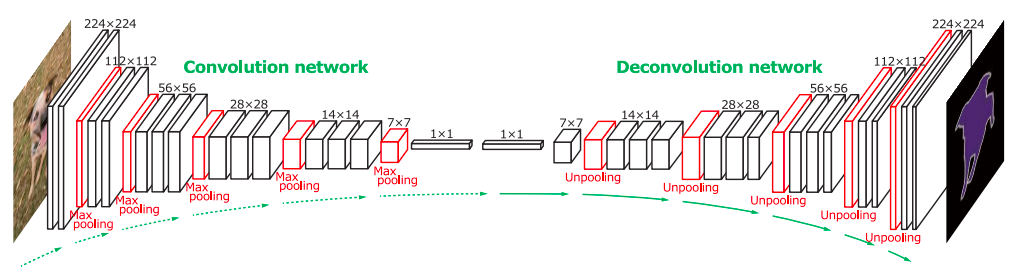
\includegraphics[width=9in]{../images/Deconv}}

\centerline{\Large [Hyeonwoo Noh et al.]}

\slide{Distortion as Probability Density}

We will assume that we have a function (deconvolution) mapping $z$ to $\hat{y}_\Phi(z)$.

\vfill
For rate-distortion autoencoders we assume a distortion function $D(y,\;\hat{y}_\Phi(z(y)))$.

\vfill
$L_1$ or $L_2$ distortion can be converted to a continuous probability density.

\vfill
$$p(y|\hat{y}) = \frac{1}{Z} \; e^{- D(y,\hat{y})}$$

\vfill
This gives a density $p_\Phi(y|z) = p(y|\hat{y}_\Phi(z))$.

\anaslide{The Reparameterization Trick}
\bigskip
$${\cal L}_{\mathrm{ELBO}}(y,\Phi,\Psi)  = \expectsub{\color{red} z \sim p_\Psi(z|y)}\;\ln\;p_\Psi(z|y) - \ln p_\Phi(z) + \lambda||y-\hat{y}_\Phi(z)||^2$$

\vfill
All variables are now continuous.

\vfill
How do we differentiate the sampling?

\vfill
\anaslide{The Reparameterization Trick}
\bigskip
$${\cal L}_{\mathrm{ELBO}}(y,\Phi,\Psi)  = \expectsub{\color{red} z \sim p_\Psi(z|y)} \;\ln\;p_\Psi(z|y) - \ln p_\Phi(z) + \lambda||y-\hat{y}_\Phi(z)||^2$$

\vfill
We note that in practice all sampling is computed by a deterministic function of (pseudo) random numbers.

\vfill
We can make this explicit.

\vfill
Model $P_\Psi(z|y)$ by $\epsilon \sim \mathrm{noise}$, $z = z_\Psi(y,\epsilon)$

\vfill
\anaslide{The Reparameterization Trick}
\bigskip
$$~\;\;\;\;\;\;\;\;\;\;\;\;\;\;\;\;\;\;\;\;\;\;\;\;\;\;\;\;\expectsub{\color{red} z \sim p_\Psi(z|y)} \;\ln\;p_\Psi(z|y) - \ln p_\Phi(z) + \lambda||y-\hat{y}_\Phi(z)||^2$$

\bigskip
becomes
$$\expectsub{\color{red} \epsilon \sim {\cal N}(0,I)} \;{\color{red} z := z_\Psi(y)+ \sigma \odot\epsilon;}\;\ln\;p_\Psi(z|y) - \ln p_\Phi(z) + \lambda||y-\hat{y}_\Phi(z)||^2$$

\slide{Decoding with $L_2$ Distortion}

Switching back to minimization, we can now rewrite the objective as

\vfill
$$\min \; \expectsub{y,\epsilon} \;\left(|z_\Psi(y,\epsilon)|_\Phi +  \frac{1}{2}\lambda||y - \hat{y}_\Phi(z_\Psi(y,\epsilon))||^2\right) - |z_\Psi(y,\epsilon)|_{\Psi,y}$$

\vfill
$$|z|_\Phi  = - \log_2 P_\Phi(z)\hspace{5em} |z|_{\Psi,y}  = - \log_2 P_\Psi(z|y)$$

\vfill
For $z$ discrete, $|z|_\Phi$ is the code length of $z(y,\epsilon)$ under an optimal code for $P_\Phi$.

\vfill
$|z|_{\Psi,y}$ is the code length for $z$ under the code for $P_\Psi(z|y)$.

\slideplain{Sampling}

$$P_\Psi(z|y) \hspace{3ex} z \hspace{3ex}  P_\Phi(z,y)$$

\centerline{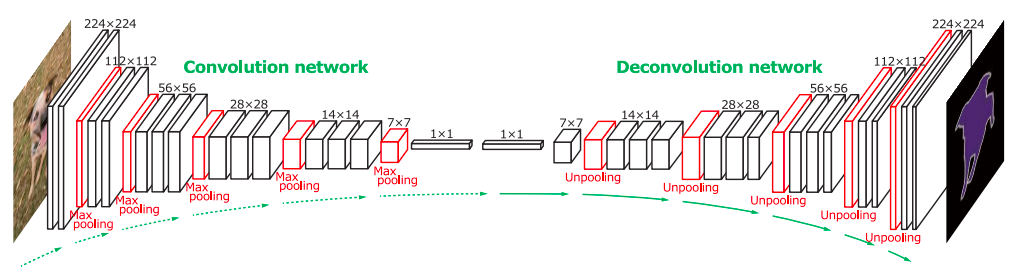
\includegraphics[width=6in]{../images/Deconv}}
\centerline{\large [Hyeonwoo Noh et al.]}

\vfill
Sampling uses just the second half ${\color{red} P_\Phi(z,y)}$.

\slide{Sampling from Gaussian Variational Autoencoders}

\vfill
\centerline{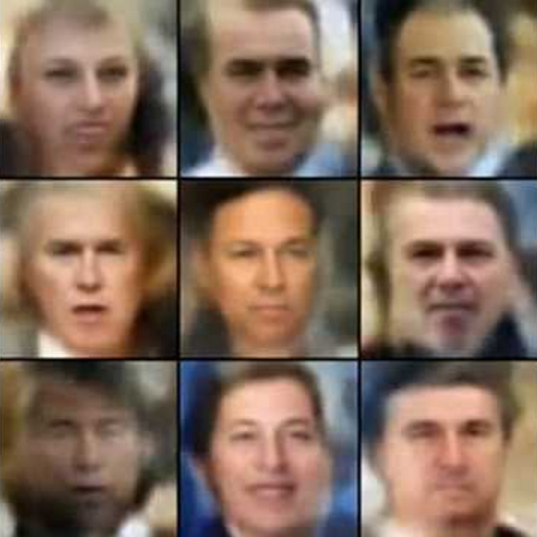
\includegraphics[width = 4in]{../images/VariationalFaces}}
\centerline{[Alec Radford]}

\slide{Why Blurry?}

A common explanation for the blurryness of images generated from VAEs is the use of $L_2$ as the distortion measure.

\vfill
It does seem that $L_1$ works better (see the slides on image-to-image GANs).

\vfill
However, training on $L_2$ distortion can produce sharp images in rate-distortion autoencoders (see the slides on rate-distortion autoencoders).

\slide{END}

}
\end{document}

